\documentclass[12pt,a4paper]{article}
\usepackage{rmpackages}																% usual packages
\usepackage{rmtemplate}																% graphic charter
\usepackage{rmexocptce}																% for DS with cptce eval

\usepackage{fontawesome}
\newcommand{\thumbsup}{\marginpar{\faThumbsOUp}}

%\cfoot{} 													% if no page number is needed
%\renewcommand\arraystretch{1.5}		% stretch table line height

\newcommand{\ritem}{\refstepcounter{enumi}\item[\writeit{} \theenumi .]}

\begin{document}

\begin{header}
TP -- Poids plume
\end{header}

\begin{multicols}{2}
\begin{center}
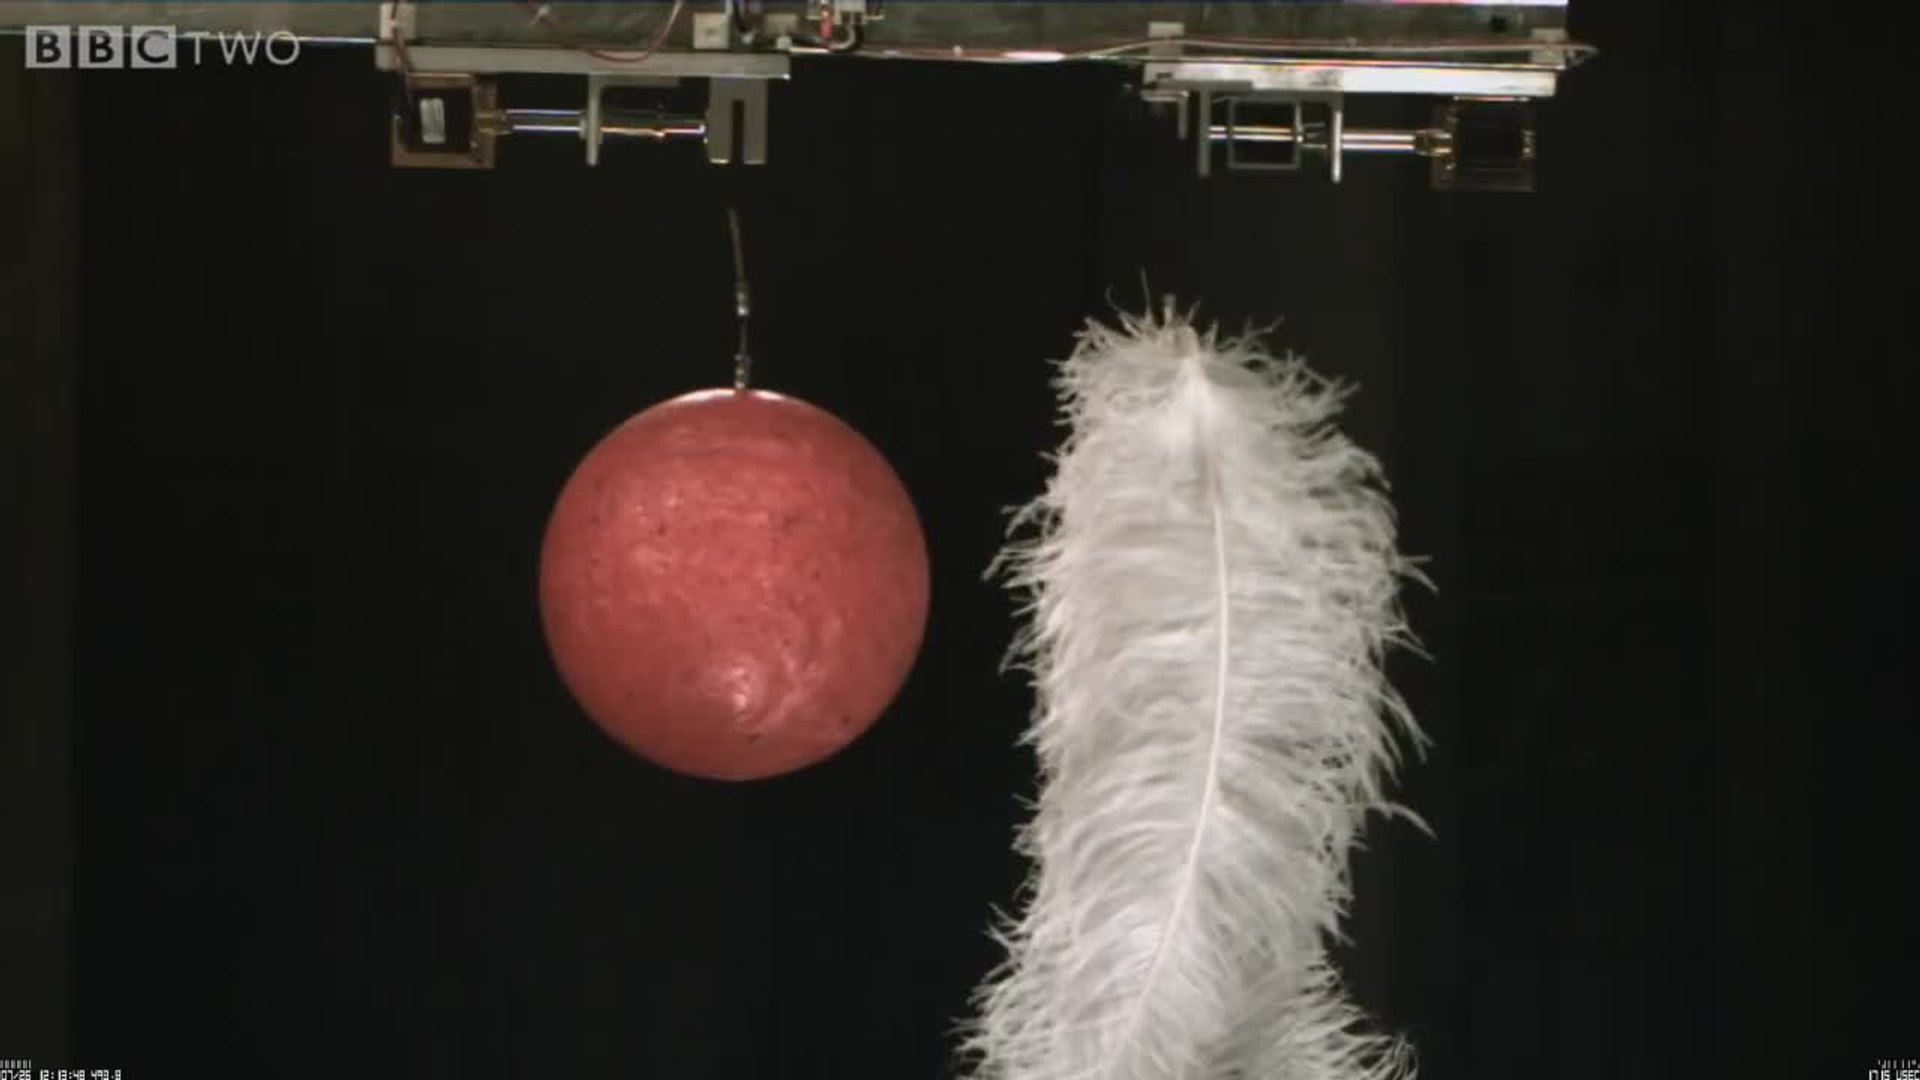
\includegraphics[width=\linewidth]{images/plumarteau.jpg}
\end{center}

Qui de la plume ou de la boule de bowling va toucher le sol en premier ?

Pour répondre à cette question, les scientifiques de la NASA ont réalisé pour nous l'expérience, sur Terre et dans une chambre à vide géante de laquelle ils ont presque entièrement retiré l'air.

Le résultat est... surprenant !
Enfin, pas pour Galilée, qui l'avait prédit dès le XVII\textsuperscript{ème} siècle...
\end{multicols}

\begin{enumerate}
\item Copier-coller tout le dossier \og TP Plume \fg{} dans votre espace de travail personnel (Ordinateur \textrightarrow{} Ma classe \textrightarrow{} Documents en consultation \textrightarrow{} Physique-Chimie) 
\end{enumerate}

\section*{L'expérience}

On souhaite tout d'abord représenter les positions successives d'une plume modélisée par un point au cours de sa chute.

\begin{enumerate}[resume]
\item Si besoin, regarder à nouveau la vidéo de l'expérience : \texttt{video\_plume}.
Vous pourrez retrouver cette vidéo ici : \href{https://youtu.be/Ha0b8n5puJM}{https://youtu.be/Ha0b8n5puJM}.

\ritem \app{} \anarai{}

Identifier le système et indiquer le référentiel choisi dans la vidéo pour étudier le mouvement de la plume.

\ritem \rco{}

Décrire le mouvement de la plume dans ce référentiel (trajectoire et vitesse).
\label{quest:trajectoire}
\end{enumerate}

\section*{Représenter la trajectoire avec Python}

Le tableau ci-dessous indique la distance entre le point de départ et la plume en fonction du temps.

\begin{center}
\begin{tabular}{|lc|c|c|c|c|c|c|c|}
\hline
\textbf{Temps} & (s) & 0{,}00 &  0{,}45 &  0{,}90 &  1{,}35 &  1{,}80 &  2{,}25 &  2{,}70 \\
\hline
\textbf{Distance} & (m) & 0{,}00 & 0{,}97 & 3{,}89 & 8{,}75 & 15{,}56 & 24{,}31 & 35{,}00 \\
\hline
\end{tabular}
\end{center}

\begin{enumerate}[resume]
\item Ouvrir le programme \texttt{chute\_libre.py} et l'exécuter 
\includegraphics[height=0.75\baselineskip]{images/edupython_execute.png}.

\ritem \app{}

À quoi correspond chacun des trois tableaux \texttt{t}, \text{X} et \texttt{Y} des lignes 7, 8 et 9 ?
\thumbsup
\end{enumerate}

\begin{appel}
\app{}
\end{appel}

\begin{enumerate}[resume]
\ritem \app{}

Quelle ligne permet de représenter graphiquement les positions successives de la plume ?

\ritem \rea{}

Calculer la vitesse moyenne de la plume pendant toute sa chute. \thumbsup
\end{enumerate}

\section*{Vecteur vitesse}

\begin{enumerate}[resume]
\ritem \rea{}

Donner les caractéristiques du vecteur vitesse $\vec{v_5}$ au point $M_5$ : direction, sens et \textbf{norme}.
\label{quest:carac_vitesse}
\end{enumerate}

\begin{appel}
\rea{} 
\end{appel}

\begin{enumerate}[resume]
\ritem \app{} \anarai{}

Supprimer le \# de la ligne 27 et exécuter le programme.
Décrire les changements observés sur le graphe.

\ritem \app{} 

Remplacer la ligne 21 par \texttt{x = 10} et décrire les changements observés sur le graphe.

\ritem \anarai{} \val{}

D'après la question précédente, expliquer à quoi correspond la valeur de \texttt{x}.
Justifier.

\ritem \anarai{} \val{}

De la même façon, expliquer à quoi correspond la valeur de \texttt{y} à la ligne 22.
Justifier.

\ritem \rea{} \val{}

Modifier les valeurs de \texttt{x}, \texttt{y}, \texttt{vx} et \texttt{vy} (lignes 21 à 25) pour représenter le vecteur vitesse $\vec{v_5}$.
Indiquer les valeurs choisies sur le compte-rendu.
\end{enumerate}

\begin{appel}
\val{}
\end{appel}

\newpage{}

\section*{Supplément 1 (2)}

\begin{enumerate}[resume]
\item \rea{} En vous aidant des lignes 27 à 33, modifier le programme pour représenter également le vecteur vitesse $\vec{v_1}$ au point $M_1$. \thumbsup
\textit{Votre programme ne devra contenir aucune valeur numérique.}

\ritem \app{} \val{} Commenter l'évolution des caractéristiques du vecteur vitesse au cours du mouvement.
Est-ce cohérent avec la question \ref{quest:trajectoire} ? Justifier.
\end{enumerate}

\begin{appel}
\end{appel}

\section*{Supplément 2 (2)}

\begin{enumerate}[resume]
\item \anarai{} \rea{} En vous aidant du programme \texttt{chute\_libre.py}, compléter le programme \texttt{saut.py} pour représenter le vecteur vitesse au point $M_4$. \thumbsup
\end{enumerate}

\begin{appel}
\end{appel}

\end{document}